\documentclass[10pt,oneside,onecolumn,letterpaper]{article}
\usepackage{graphicx}
\usepackage{xcolor}
\usepackage[hidelinks]{hyperref}
\usepackage{booktabs}
\usepackage{adjustbox}

\usepackage[top=.5in, bottom=1in, left=.5in, right=.7in]{geometry}

\usepackage{fontspec}
\setmainfont{Arial}

\begin{document}

%%
% THIS IS THE HEADER
%%
\noindent\colorbox{black}{
\begin{minipage}[c]{.99\linewidth}
  \vspace{.4cm}
  \Large{\color{white}{\textbf{\hspace{.3cm}University of Massachusetts Boston}}}
  \begin{flushright}
    \vspace{-1.2cm}
    
\includegraphics[width=3cm]{gfx/cs460.png}
  \end{flushright}
\end{minipage}
}

%%
% CONTENT STARTS HERE
%%

\vspace{.5cm} % add some space

\noindent\textbf{CS460 Fall 2019} \\
\textbf{Name:} Jared Barresi \\
\textbf{Student ID:} 00974358 \\
\textbf{Due Date:} 12/02/2019

\section*{Assignment 10: glTF!}

\textbf{We will load our favorite mesh from a file and then convert it to1 a valid glTF file.} You can choose if you want to do this assignment in JavaScript or in Python. In class, we used Python (see our colab from class \url{https://cs460.org/shortcuts/33/})

\vspace{.5cm} % add some space

\begin{center}
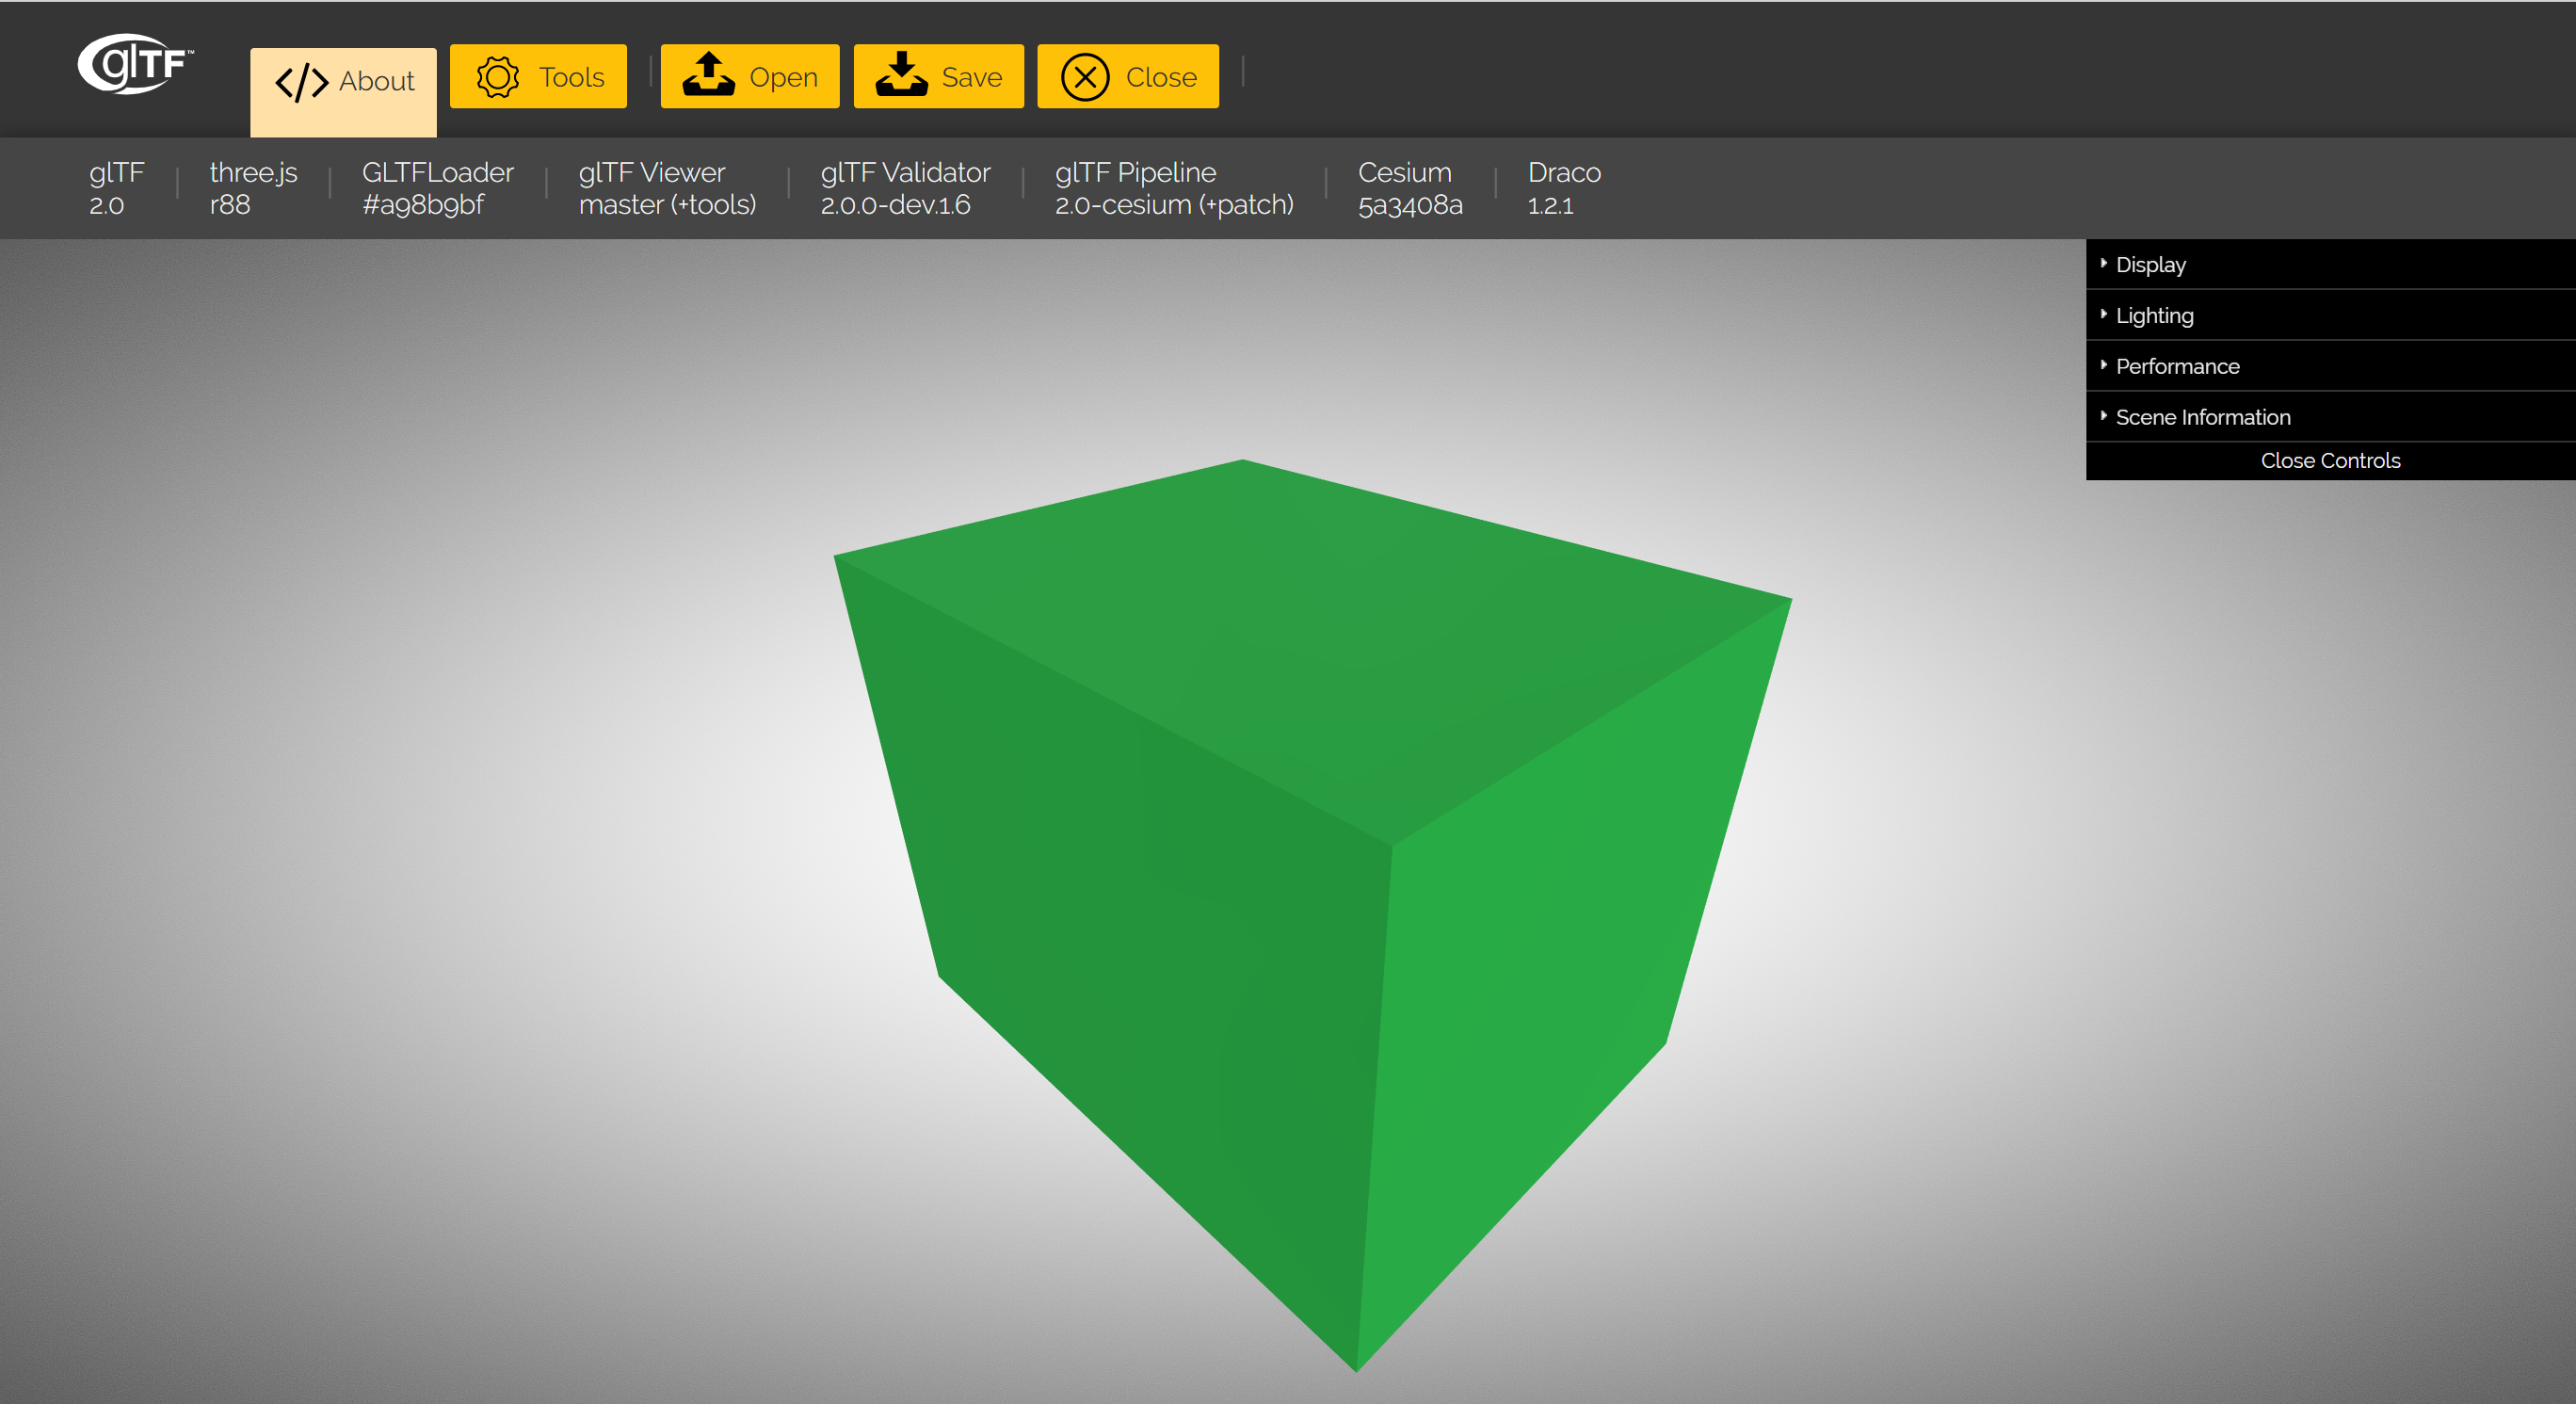
\includegraphics[width=.5\textwidth]{gfx/Screenshot-1.png}
\end{center}

\vspace{.5cm}

\noindent\textbf{Starter code for assignment 10.} After pulling from upstream, there is the folder \url{10} in your fork. This folder contains an \url{index.html} file that uses JavaScript to make glTF JSON. This folder also contains a \url{gltf.py} script that you can run with \url{python} \url{gltf.py} to output the glTF JSON. As a start for this assignment, both versions create an identical valid glTF JSON structure holding a single triangle (see screenshot above).

\vspace{.5cm}


\noindent\textbf{Part 1 (1 points):} Please decide which language you will use: JavaScript or Python. Python might be a bit easier to load and parse an existing file---with JavaScript we need to use Ajax to load the existing mesh and parse it (or as option 3: use a Three.js loader and grab the vertices/indices from there). For parsing files with Python look here: \url{https://tutorial.eyehunts.com/python/python-read-file-line-by-line-readlines/} For using Javascript and Ajax look here: \url{https://developer.mozilla.org/en-US/docs/Web/API/XMLHttpRequest/Using_XMLHttpRequest}.

\vspace{.3cm}

\textbf{Choice:} JavaScript

\vspace{.5cm}

\noindent\textbf{Part 2 (15 points):} Load a mesh from an external file. A .PLY or .OBJ file might be the easiest to parse.

\vspace{.5cm}

\noindent\textbf{Part 3 (20 points):} Parse all vertices from the loaded mesh and create the VERTICES array and base64 code.

\vspace{.5cm}

\noindent\textbf{Part 4 (20 points):} Parse all indices from the loaded mesh and create the INDICES array and base 64 code.

\vspace{.5cm}

\noindent\textbf{Part 5 (10 points):} Calculate all required fields for the glTF file (as we did in class) and generate the glTF JSON code. Store the glTF JSON code in a glTF file.

\vspace{.5cm}

\noindent\textbf{Part 6 (5 points):} Please make sure the glTF file is valid using \url{http://github.khronos.org/glTF-Validator/}.

\vspace{.5cm}

\noindent\textbf{Part 7 (5 points):} Visualize the glTF file using \url{https://gltf.insimo.com/}. You might have to choose the wireframe display option since the glTF file does not include material (Display -> Wireframe, in the dat.GUI). \textbf{Please replace the screenshot above.}

\vspace{.5cm}

\noindent\textbf{Part 8 (5 points):} Add the glTF file to your fork.

\vspace{.5cm}

\noindent\textbf{Part 9 (10 points):} Choose a final project---either an existing one from \url{https://cs460.org/assignments/final/} or a new one. Please list the project here and in the link. If working as a team, assemble your team and list the team members below and in the link. 

\vspace{.5cm}



\noindent\textbf{XTK for Android (+Accessibility)} Android application that provides a bridge (in javascript) to all the Android API's to use with XTK. Created a custom bridge framework, using the platform Droidscript. \url{http://www.androidscript.org} Some api "features" implemented include: Button/Slider input, Voice Recognition, Sensor Recognition. (All Prior elements can be used to generate XTK objects, and change their properties) (+ more!).
\vspace{1cm}


\url{https://github.com/hltdev8642/cs460student/tree/master/final-project}

\vspace{3cm}

\noindent\textbf{Part 10 (9 points):} Make sure this PDF and your glTF file are in your fork on github. Then, please send a pull request.

\vspace{.5cm}


\vspace{3cm}

\noindent\textbf{Bonus (33 points):}

\vspace{.5cm}

\noindent\textbf{Part 1 (15 points):} Please add any kind of material to the glTF file. For this, you would have to read the specs or google for examples :)
[x]Has a color (+ texture)
\vspace{.5cm}

\noindent\textbf{Part 2 (18 points):} Write THREE.js code that displays your glTF file using the \url{THREE.GLTFLoader}.

\end{document}
